\documentclass{article}
\input{../../../../../../LaTex/preamble/preamble_article.tex}

\begin{comment}
    重复语句
    \subsubsection{}
    \includegraphics[width=50em,keepaspectratio]{}

    \begin{itemize}
        \item 错选:\quad
        \item 正解:\quad
        \item 总结:\quad
        \item 扩展:\quad
    \end{itemize}

\end{comment}


\title{热学总复习习题及作业}
\author{学生:杨凤 \quad 教师: 马祥芸}

\begin{document}
\maketitle
\tableofcontents
\newpage

\section{课堂习题}

\subsection{图像计算}
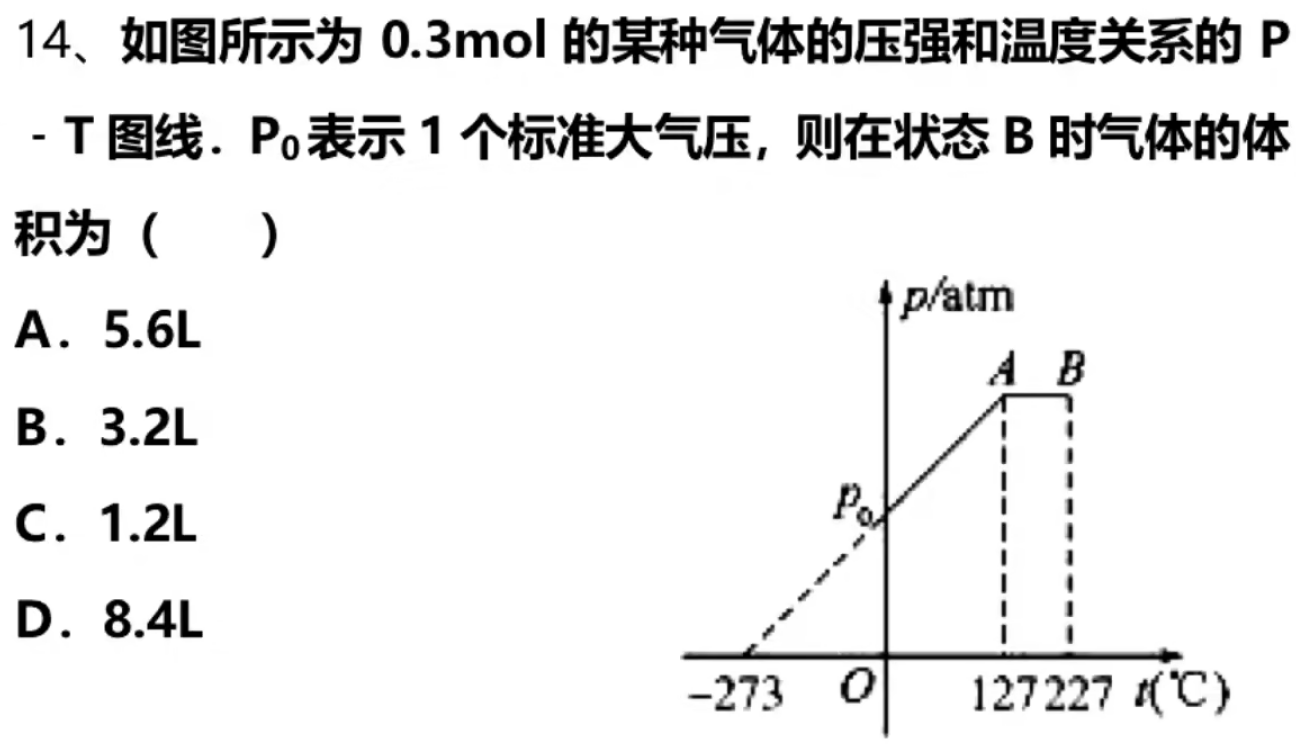
\includegraphics[width=0.55\textwidth,keepaspectratio]{./pictures/2.3-3.png}

\vspace{2em}

\subsection{动力学问题}
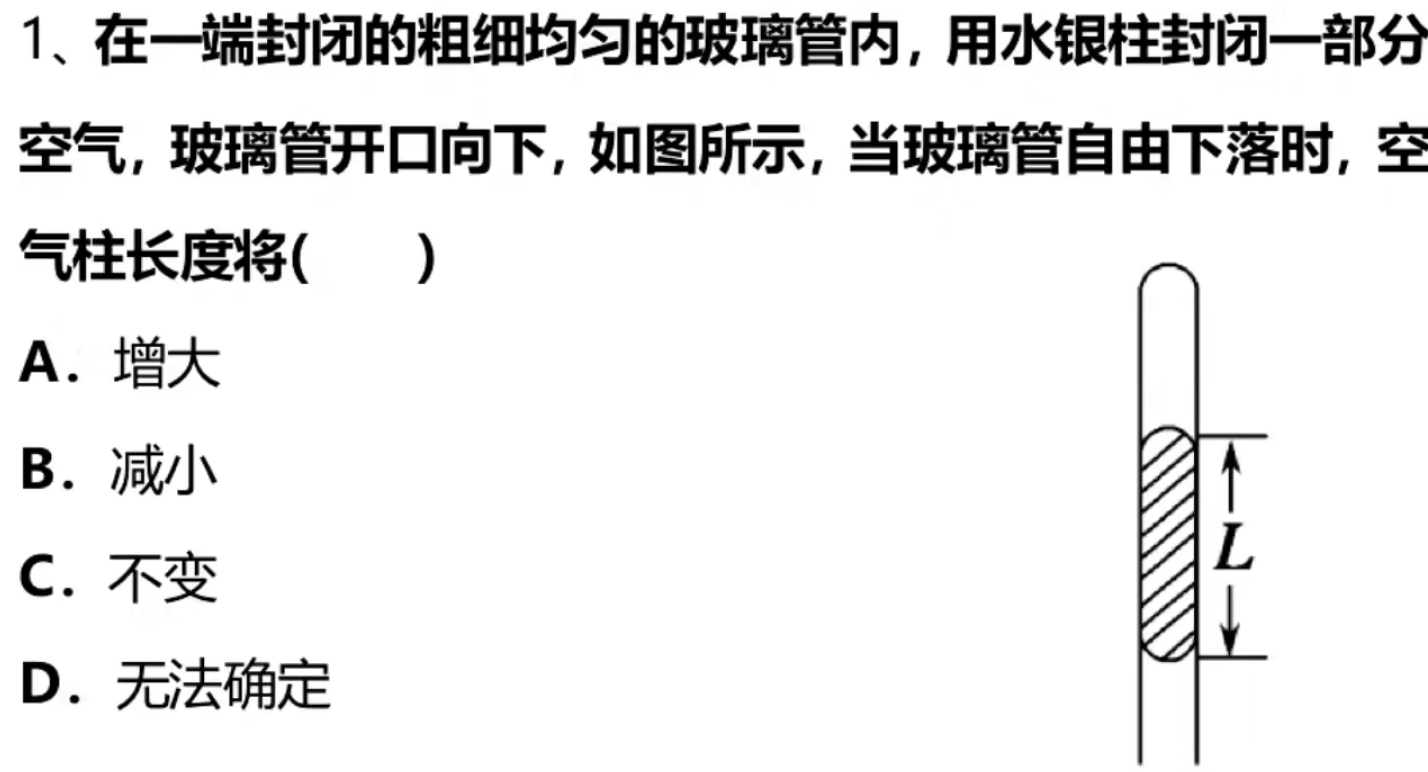
\includegraphics[width=0.55\textwidth,keepaspectratio]{./pictures/2.3-4.png}

\vspace{2em}

\subsection{移动分析}
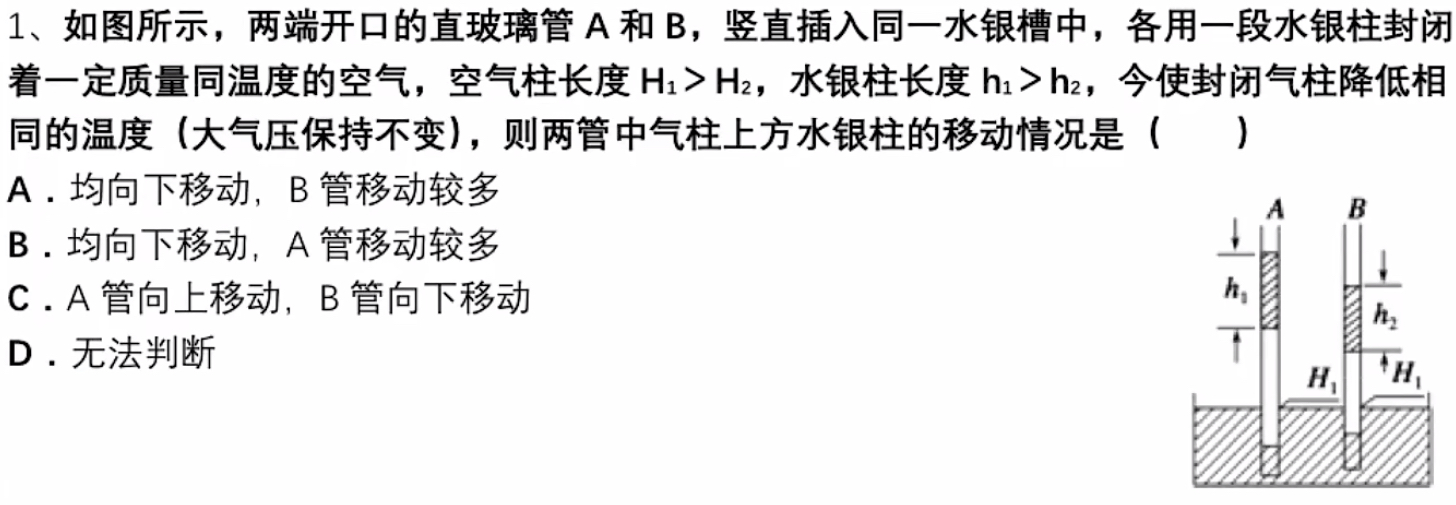
\includegraphics[width=0.95\textwidth,keepaspectratio]{./pictures/2.3-7.png}

\vspace{2em}

\subsection{充气问题}
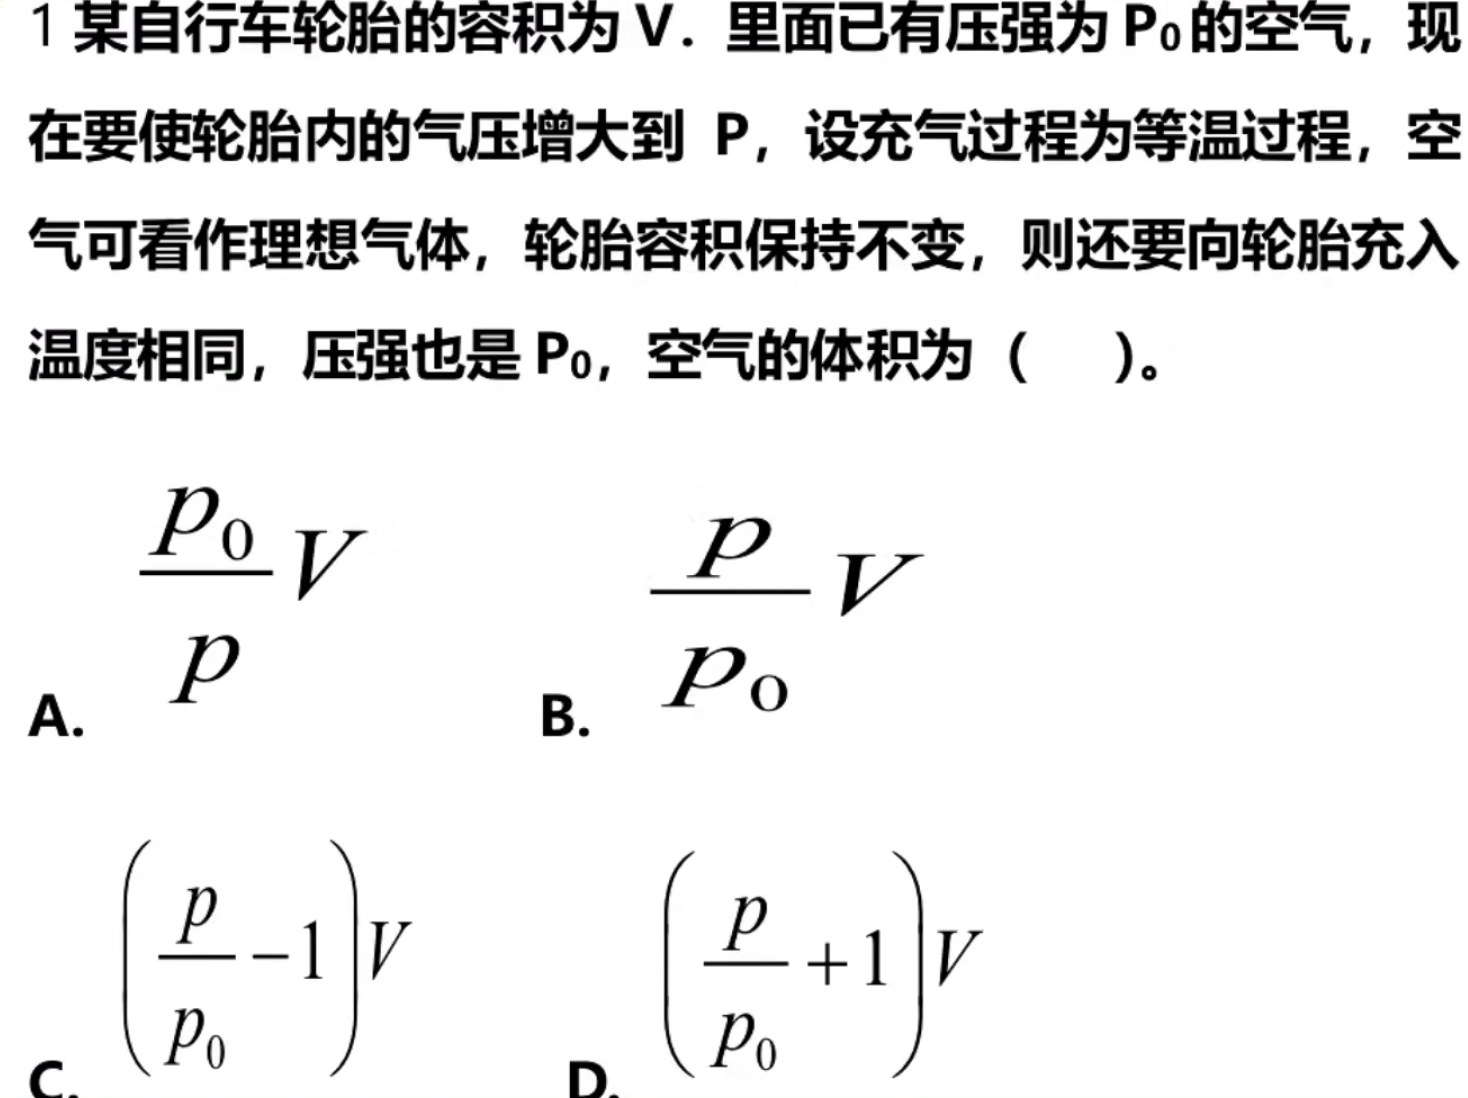
\includegraphics[width=0.55\textwidth,keepaspectratio]{./pictures/2.3-10.png}

\vspace{2em}

\subsection{图像问题}
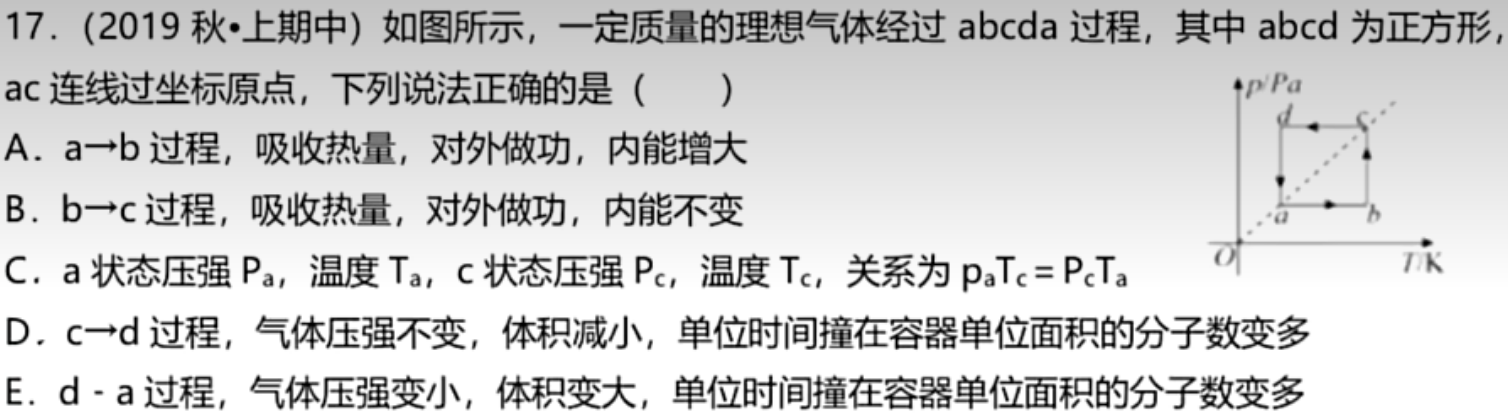
\includegraphics[width=0.95\textwidth,keepaspectratio]{./pictures/2.3-33.png}

\newpage

\section{作业}

\subsection{三连通器}
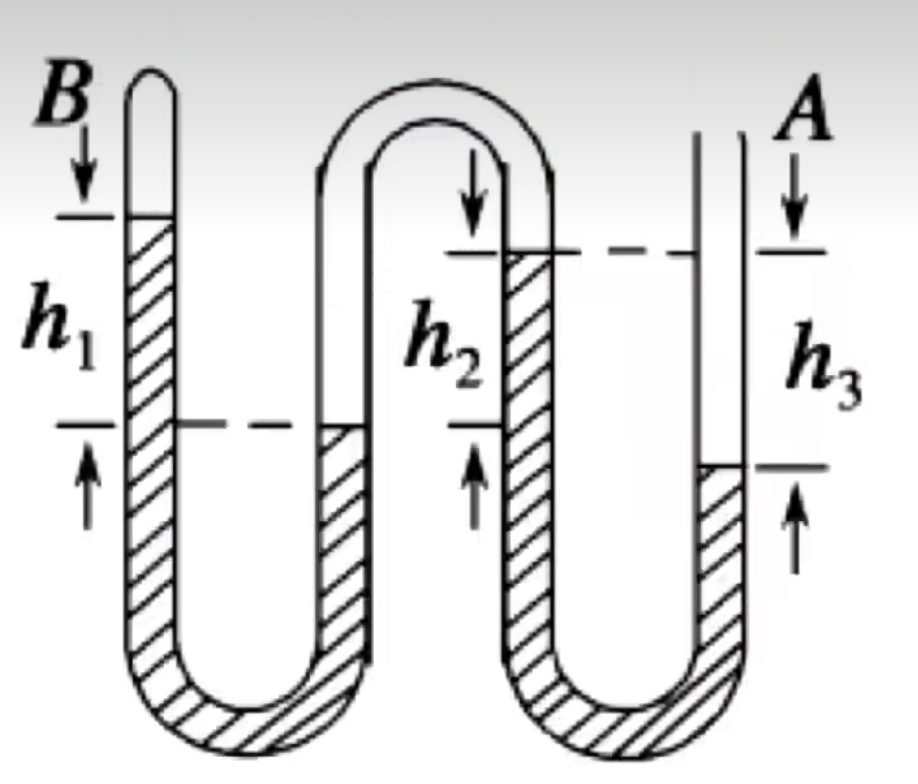
\includegraphics[width=0.55\textwidth,keepaspectratio]{./pictures/2.3-1.png}

\vspace{2em}

\subsection{液泡}
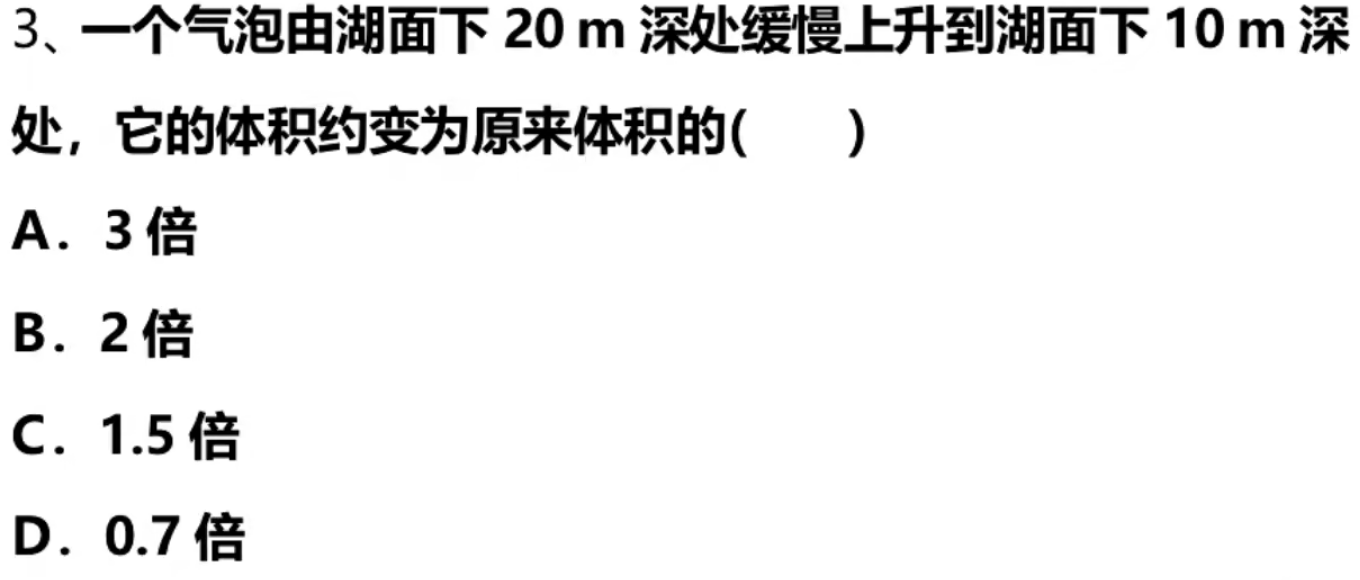
\includegraphics[width=0.55\textwidth,keepaspectratio]{./pictures/2.3-2.png}

\vspace{2em}

\subsection{挤压问题}
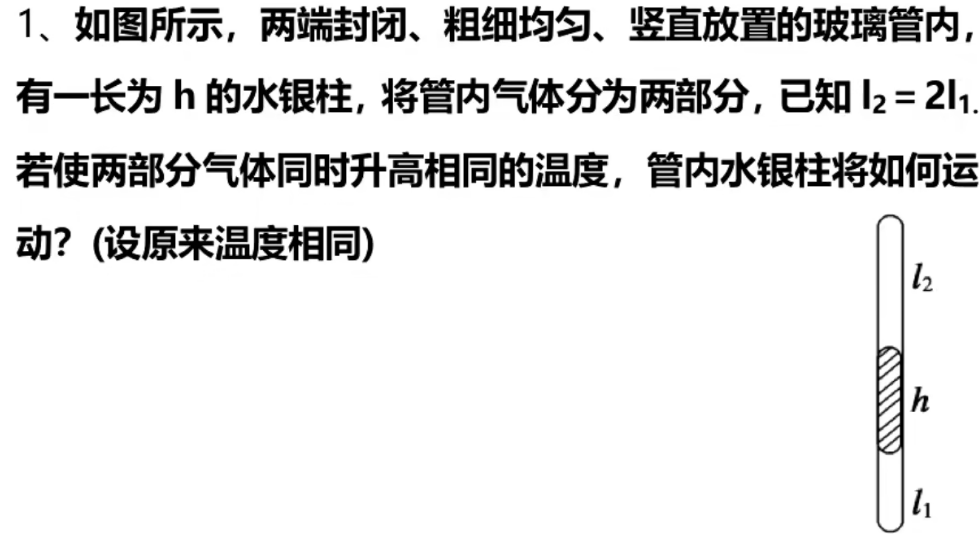
\includegraphics[width=0.55\textwidth,keepaspectratio]{./pictures/2.3-5.png}

\vspace{2em}

\subsection{移动综合}
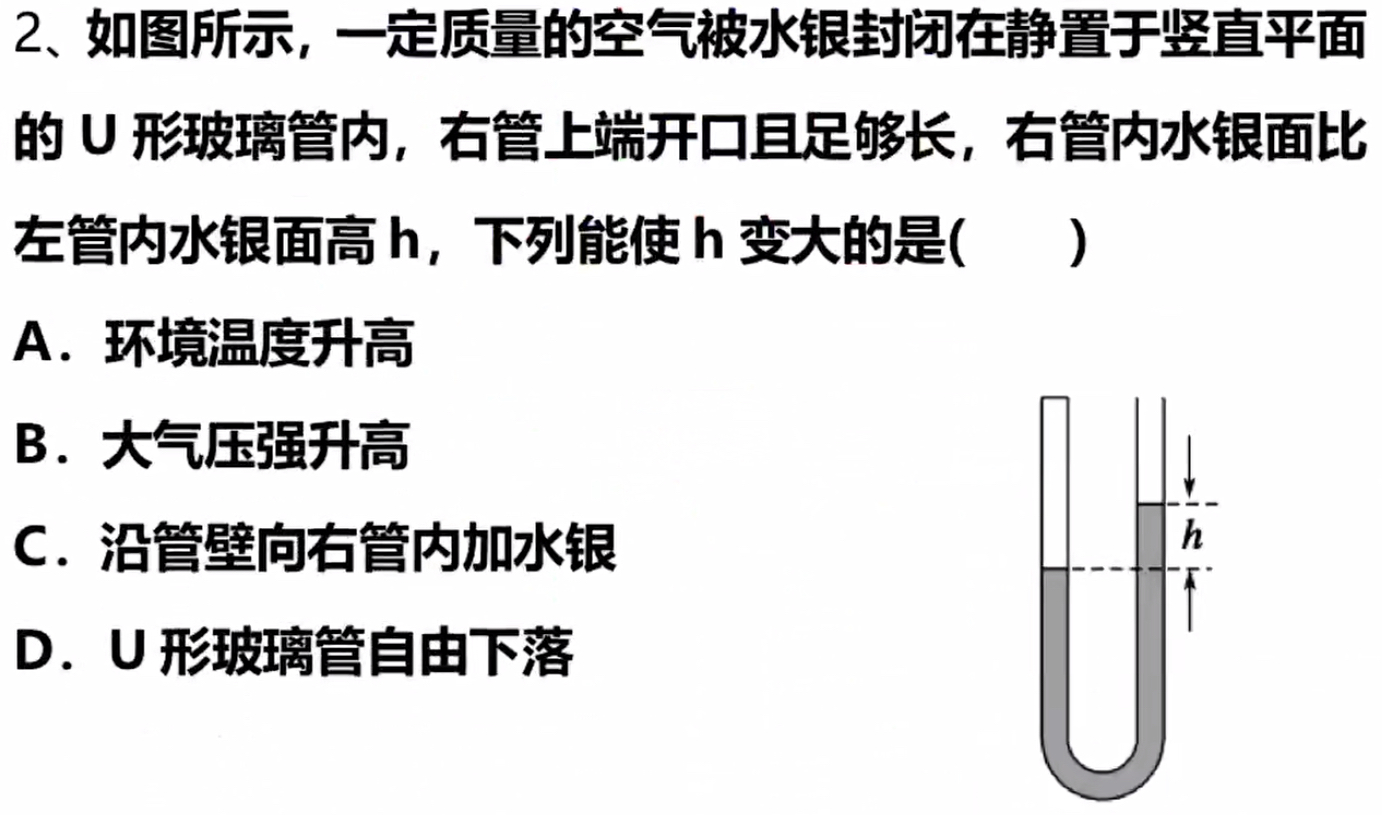
\includegraphics[width=0.55\textwidth,keepaspectratio]{./pictures/2.3-9.png}

\vspace{2em}

\subsection{图像分析}
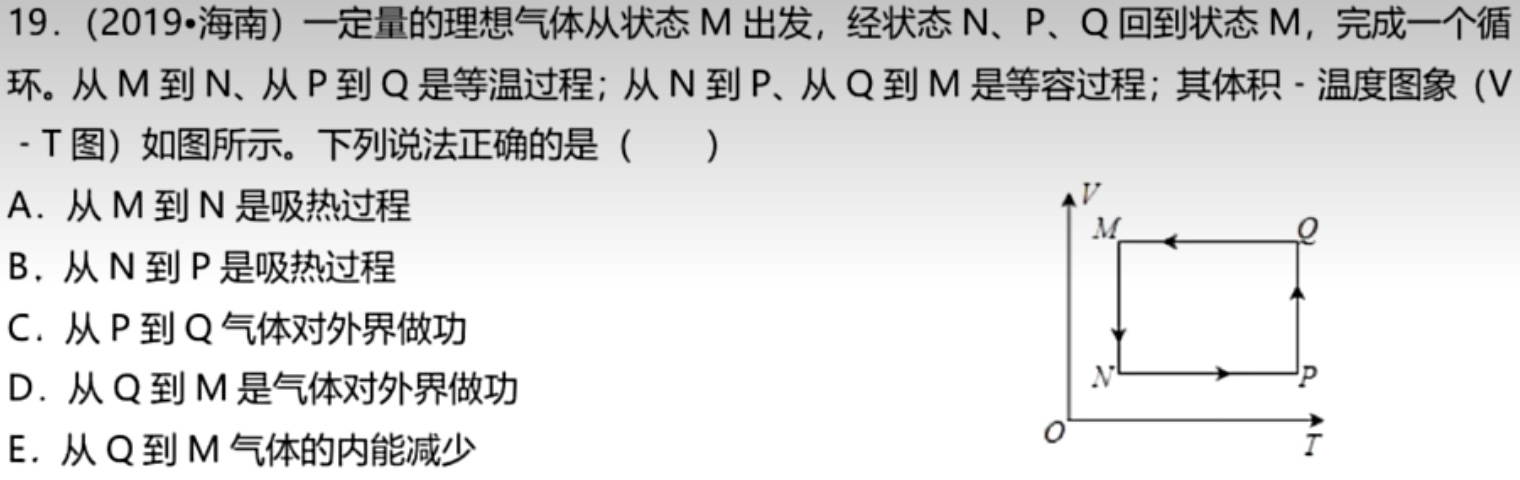
\includegraphics[width=0.95\textwidth,keepaspectratio]{./pictures/2.3-35.png}

\vspace{2em}

\subsection{图像分析}
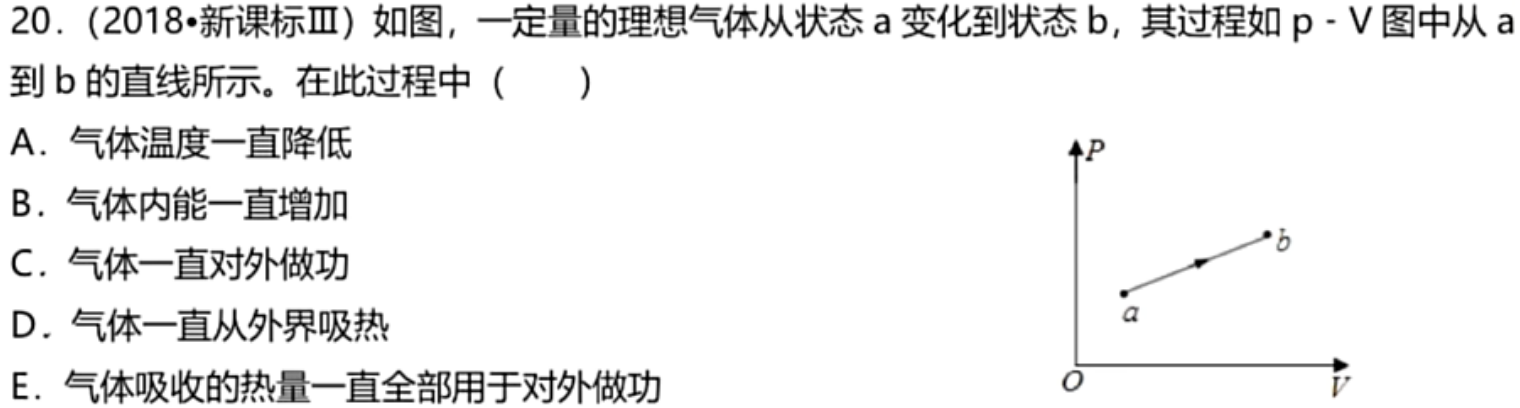
\includegraphics[width=0.95\textwidth,keepaspectratio]{./pictures/2.3-36.png}

\vspace{2em}

\subsection{放气问题}
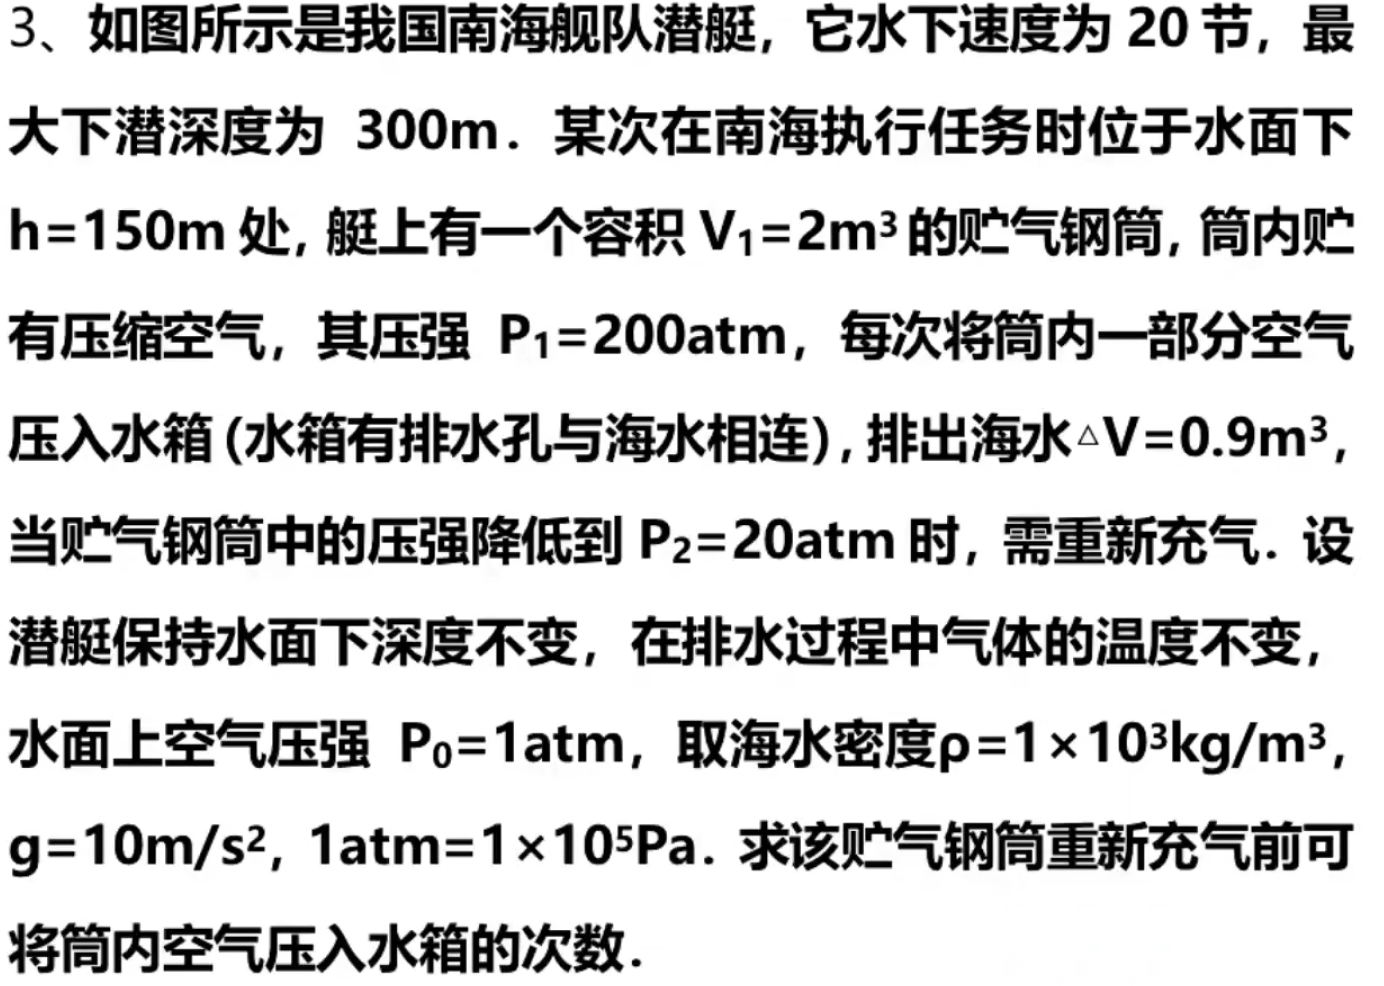
\includegraphics[width=0.55\textwidth,keepaspectratio]{./pictures/2.3-11.png}

\vspace{5em}

\subsection{热一计算}
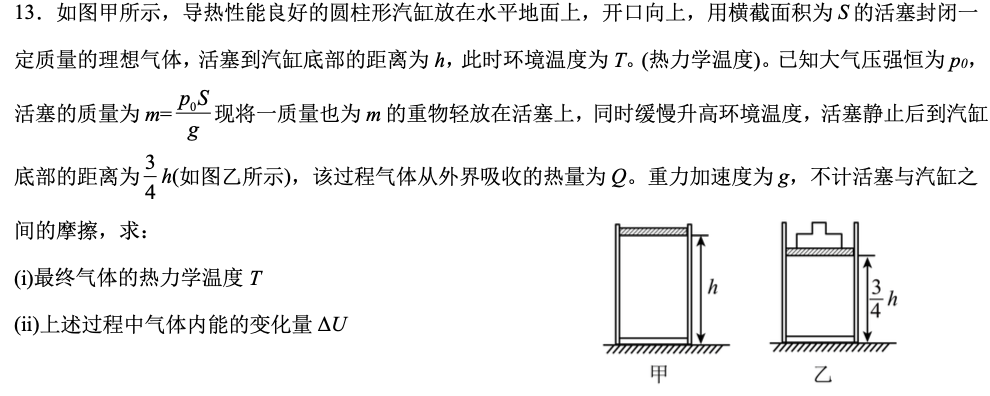
\includegraphics[width=0.95\textwidth,keepaspectratio]{./pictures/2.3-39.png}

\newpage

\section{答案及解析}
\subsection{课堂习题}
\subsubsection{}
\begin{itemize}
    \item 正解:\quad $D$
    \item 总结:\quad 首先应该向左平移$y$轴,使得横坐标换算成开尔文温度.

          \hspace{3.3em}新的坐标系下,斜线$OA$满足$P = \frac{C}{V}T$斜率为定值,因此为等容过程.

          \hspace{3.3em}$T = 273k$时直线过$P_{0}$,此时气体体积为$22.4L$,因此$V_{A} = 22.4L$
          
          \hspace{3.3em}横线$A \ra B$为等压过程,计算温度之比即可求得$V_{B}$
\end{itemize}

\vspace{2em}

\subsubsection{}
\begin{itemize}
    \item 正解:\quad $B$
    \item 总结:\quad 动力学问题主要在于分析好初末态,同时列受力分析方程.

          \hspace{3.3em}初态$PS + mg = P_{0}S$,末态自由落体加速度为$g$

          \hspace{3.3em}$P^{'}S + mg - P_{0}S = ma = mg \lra P^{'} = P_{0}$液柱上方压强增大,因此液柱上方体积减小
\end{itemize}

\vspace{2em}

\subsubsection{}
\begin{itemize}
    \item 正解:\quad $B$
    \item 总结:\quad

          \hspace{3em}\begin{minipage}{0.88\textwidth}
              此题不能使用等体过程的$\frac{\triangle P}{\triangle T}$进行分析

              两试管各自独立,区别于等体两气挤压问题(作用对象为同一个液柱)

              但两试管均连通大气$P_{0} + h_{1} = P_{A} \quad P_{0} + h_{2} = P_{B}$

              因此可视作等压过程,同有过原点的直线$V = \frac{1}{P} T \lra \frac{V}{T} = \frac{\triangle V}{\triangle T}$

              $V_{A} = \frac{\triangle V_{A}}{\triangle T} T \quad V_{A} > V_{B} (\text{两者均为负数,液柱下移})\lra \triangle V_{A} > \triangle V_{B}$
          \end{minipage}
\end{itemize}

\vspace{2em}

\subsubsection{}
\begin{itemize}
    \item 正解:\quad $C$
    \item 总结:\quad

          \hspace{3.2em}\begin{minipage}{0.88\textwidth}
              \begin{align*}
                                        & \text{由于是限容问题,本质上是求}:\triangle n \llra \triangle V                                          \\
                  P_{0}V                & = n_{1}RT                                                                                   \\
                  PV                    & = n_{2}RT \quad \lra \quad (P-P_{0})V = (n_{2} - n_{1})RT                                   \\
                  P_{0} \triangle V     & = \triangle n RT = (n_{2} - n_{1})RT  \quad \lra \quad \triangle V = (\frac{P}{P_{0}} - 1)V \\
                                        & \text{或者使用一个方程要求: 原状态 \, + \, 打入气 = 末状态}                                                    \\
                  P_{0} V + P_{0} V_{0} & = PV \quad \lra \quad \triangle V = (\frac{P}{P_{0}} - 1)V
              \end{align*}
          \end{minipage}

\end{itemize}

\vspace{2em}

\subsubsection{}
\begin{itemize}
    \item 正解:\quad $ACD$
    \item 总结:\quad $D \, E$选项的判断体积越小,那么显然单位体积内的分子数上升,碰撞容器壁的概率会上升
\end{itemize}

\vspace{2em}

\subsection{课后作业}
\subsubsection{}
\begin{itemize}
    \item 正解:\quad $P_{B} = P_{A} + \rho g (h_{3} - h_{1}) $
    \item 总结:\quad 前两管: $ P_{B} + \rho g h_{1} = P_{C}\text{,后两管} P_{C} + \rho g h_{3} = P_{0}$
\end{itemize}

\vspace{2em}

\subsubsection{}
\begin{itemize}
    \item 正解:\quad $C$
    \item 总结:\quad 外界大气压的作用应该被计算进去
\end{itemize}

\vspace{2em}

\subsubsection{}
\begin{itemize}
    \item 正解:\quad 向上移动
    \item 总结:\quad 三个状态参量中,真正使得液柱移动的物理量是$P$,在查理定律中$\frac{P}{T} = \frac{C}{V}$

          \hspace{3.3em}升温瞬间可视为\textbf{等体}过程,因此函数为过原点的直线可得$\frac{P}{T} = \frac{\triangle P}{\triangle T}$

          \hspace{3.3em}$ \triangle P_{1} = \frac{P_{1}}{T_{1}} \triangle T = \frac{C}{V_{1}} \triangle T $

          \hspace{3.3em}$ V_{2} = 2 V_{1}  \quad \lra \triangle P_{1} > \triangle P_{2}$
\end{itemize}

\vspace{2em}

\subsubsection{}
\begin{itemize}
    \item 正解:\quad $ACD$
    \item 总结:\quad

          \hspace{3em}\begin{minipage}{0.88\textwidth}
              \begin{enumerate}[label = (\Alph*)]
                  \item 通常当多个变量发生变化,优先假设$V$不变,因此瞬态满足$\frac{P}{T} = \frac{\triangle P}{\triangle T} = C$

                        $P = P_{0} + h$方程右边暂时不变,环境温度上升$\triangle T > 0 \lra \triangle P > 0$,压强$P$增大

                        虽然体积$V$减小导致$h$又下降,但稳态总有$P$变大,因此需要$h$变大,$A$正确
                  \item $P_{0}$上升,$P$上升,等温条件下$V$下降,因此试管左边的体积下降导致$h$变小
                  \item 可以从两个角度思考,只要持续往里加水银,必然会使得液面高$h$上升

                        另一个角度,瞬态时$h$变大,$P$变大,$V$减小,末态方程$P^{'} = P_{0} + h^{'}$

                        结果上必然有$P^{'}>P$,因此$h$变大
                  \item 自由落体需要列动力学方程,$P_{0}S + mg - P^{'}S = mg \lra P^{'} = P_{0}$压强变小,体积变大,$h$上升
              \end{enumerate}
          \end{minipage}
\end{itemize}

\vspace{2em}

\subsubsection{}
\begin{itemize}
    \item 正解:\quad $BCE$
\end{itemize}

\vspace{2em}

\subsubsection{}
\begin{itemize}
    \item 正解:\quad $BCD$
    \item 总结:\quad $E$选项注意能量的转化角度,热量一部分转化为对外做功一部分作为内能储存
\end{itemize}

\vspace{2em}

\subsubsection{}
\begin{itemize}
    \item 正解:\quad $25$次
    \item 总结:\quad 主要在于排出气体的压强与水压+大气压平衡,是恒压为$1 \, atm + P_{\text{水}}$,其中$P_{\text{水}} = 15 \, atm$
\end{itemize}

\vspace{2em}

\subsubsection{}
\begin{itemize}
    \item 正解:\quad $(1) \, \frac{9}{8} \, T \quad (2) \,  Q + \frac{3}{4}P_{0}Sh$
    \item 总结:\quad 做功计算是准静态过程,此过程中所有的力视为不变
    
    \hspace{3.2em}受力分析包括: 物块与活塞重力,大气压力
\end{itemize}

\end{document}